\section{Результаты}

\subsection{Поле напряжений у границы и его затухание}

На рис.~\ref{fig:sigma} показано, как напряжение в матрице алюминия меняется
с расстоянием $r$ от плоскости границы в двух ячейках границы
(раздел~2.1): в контрольной, где гребень не деформирован, и в ячейке, где
гребень удлинён вдоль направления поля на $\varepsilon = 1{,}94\cdot10^{-3}$
и удерживается в этом состоянии (раздел~2.2). Деформированная ячейка
построена из релаксированной контрольной смещением атомов гребня и затем
минимизирована, так что две ячейки различаются только деформацией гребня.
Матрица разбита на слои толщиной 4~\AA{}, параллельные границе; шесть
компонент тензора напряжений усреднены по атомам алюминия каждого слоя, и
лишь из усреднённого тензора образованы инварианты (раздел~2.4).
Используются два усреднения. Первое охватывает всю ячейку по $x$ и $y$, то
есть область как над гребнем, так и рядом с ним; второе ограничено окном
шириной 20~\AA{} вокруг оси гребня --- это напряжение, которое матрица
испытывает непосредственно над включением. Гребень --- полуэллиптический
выступ включения с полуосями 35~\AA{} вдоль $x$ и 20~\AA{} вдоль $z$
(рис.~\ref{fig:cell}) --- имеет вершину при $r = 20$~\AA{}, так что над
вершиной расстояние до ближайшей поверхности включения равно
$d = r - 20$~\AA{}.

\begin{figure}[!htbp]
\centering
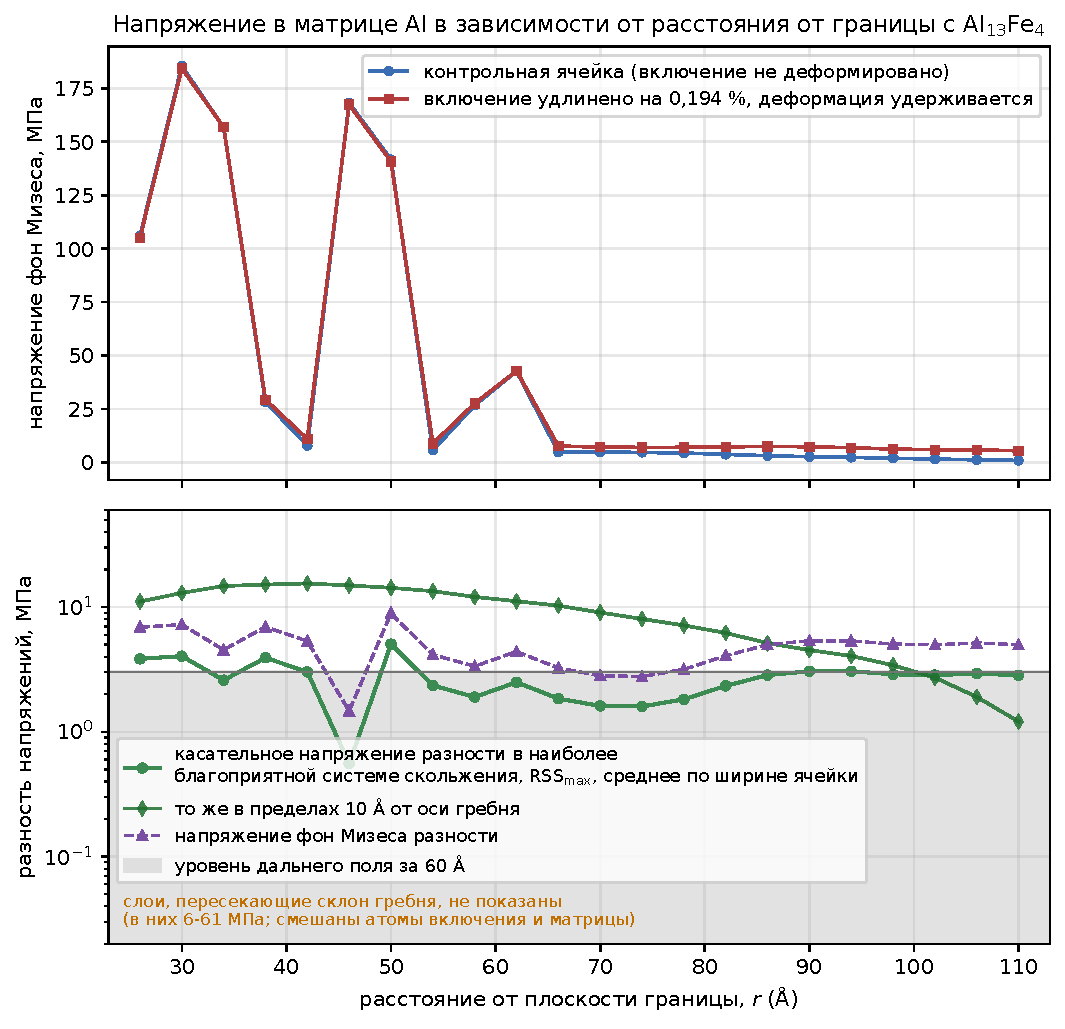
\includegraphics[width=0.80\linewidth]{fig_sigma_profile_ru}
\caption{Напряжение в матрице алюминия в зависимости от расстояния $r$ от
плоскости границы в двух ячейках границы (91\,428 атомов): в контрольной
ячейке с недеформированным гребнем и в ячейке, где гребень удлинён вдоль
направления поля на 0{,}194\% и удерживается при этой деформации. Матрица
разбита на слои толщиной 4~\AA{}, параллельные границе; шесть компонент
тензора напряжений усредняются по атомам алюминия каждого слоя, и лишь
затем из усреднённого тензора образуются инварианты. Сверху: напряжение фон
Мизеса в каждой из ячеек; 100--190~МПа непосредственно над вершиной гребня,
присутствующие в обеих ячейках, --- это напряжение когерентности сцеплённой
границы между двумя кристаллами с разными межатомными расстояниями; кривые
совпадают. Снизу: разность $\Delta\sigma_{ij} = \sigma_{ij}(\varepsilon) -
\sigma_{ij}(0)$ как касательное напряжение, спроецированное на наиболее
благоприятную из двенадцати систем скольжения ГЦК-алюминия,
$\mathrm{RSS}_{\max}$, в среднем по всей ширине ячейки (кружки) и в
пределах 10~\AA{} от оси гребня (ромбы), а также напряжение фон Мизеса
разностного тензора. Затенённая область отмечает напряжения ниже 3~МПа: уровень среднего по
ширине за 60~\AA{} с его разбросом, $2{,}5 \pm 0{,}5$~МПа, разрешающая
способность расчёта для длинноволновых деформаций слоя. Слои на уровне склонов гребня, лежащие ближе
к плоскости границы, чем его вершина, опущены: там $r$ не является
расстоянием до поверхности включения, и слои содержат атомы включения.
Профиль обрывается в 20~\AA{} под свободной поверхностью слоя.}
\label{fig:sigma}
\end{figure}

Верхняя панель даёт напряжение фон Мизеса (раздел~2.4) в каждой ячейке. Две
особенности контрольной кривой требуют прямого объяснения, поскольку они
присутствуют без всякой заданной деформации. Во-первых, в слоях
непосредственно над вершиной гребня напряжение составляет 100--190~МПа, а
на уровне склонов гребня достигает 0{,}8--2{,}2~ГПа. Это напряжение
когерентности границы. Алюминий и Al$_{13}$Fe$_4$ --- разные кристаллы с
разными межатомными расстояниями; через границу их атомы взаимодействуют
тем же межатомным потенциалом, что и внутри каждого из кристаллов, без
каких-либо искусственных связей (раздел~2.1), так что граница сцеплена и
проскальзывать не может, а атомы по обе её стороны смещены с тех положений,
которые отвела бы им собственная решётка. За $r \approx 65$~\AA{} это напряжение падает ниже 10~МПа, а за 95~\AA{}
--- ниже 2~МПа; чередование
соседних слоёв ближе к вершине отражает изгиб атомных плоскостей над ней:
слой толщиной 4~\AA{} захватывает там одну или две плоскости с разными
напряжениями. Это напряжение существует независимо от того, деформирован
гребень или нет: две кривые верхней панели совпадают, напряжение фон Мизеса
разностного тензора над вершиной не превышает 9~МПа. Именно поэтому действие
заданной деформации всюду измеряется как разность между деформированной и
контрольной ячейками, слой за слоем. Во-вторых, профиль обрывается в
20~\AA{} под свободной поверхностью алюминиевого слоя, лежащей при
$r = 129$~\AA{}: в слоях ближе к поверхности поатомное напряжение
определяется самими поверхностными слоями.

Нижняя панель показывает саму разность
$\Delta\sigma_{ij}(r) = \sigma_{ij}(r;\varepsilon) - \sigma_{ij}(r;0)$ ---
ту величину, которая, согласно механизму работы [5], должна превышать
предел текучести матрицы. Все пороги движения дислокаций в разделе~3.2
выражены через разрешённое касательное напряжение, поэтому и разность
выражена так же. $\mathrm{RSS}_{\max}$ (раздел~2.4) вычисляется из разностного тензора, а не как разность значений фон Мизеса,
которая инвариантом $\Delta\sigma_{ij}$ не является; рядом построено
напряжение фон Мизеса самого разностного тензора. В каждом слое над
вершиной, кроме одного, наиболее благоприятной оказывается система $(111)[1\bar{1}0]$ ---
плоскость скольжения, параллельная границе, и направление $x$, вдоль
которого скользят дислокации раздела~3.2; для неё разрешённый сдвиг есть
просто компонента $\Delta\sigma_{xz}$. Исключение --- слой при
$r = 46$~\AA{}, где два вклада почти компенсируют друг друга и наибольшее
из двенадцати значений, 0{,}6~МПа, приходится на $(111)[01\bar{1}]$.

Над осью гребня разрешённое касательное напряжение составляет 11--15~МПа
от вершины до $d \approx 30$~\AA{} с максимумом 15~МПа при $d = 22$~\AA{};
далее оно спадает: 10~МПа при $d = 46$~\AA{}, 5~МПа при $d \approx 65$~\AA{}
и 2~МПа при $d \approx 85$~\AA{}. В среднем по всей ширине ячейки та же
разность много меньше, не более 5~МПа (максимум 5{,}0~МПа при $r = 50$~\AA{}, один слой при 0{,}6~МПа),
потому что гребень занимает меньше половины ширины, а сдвиг рядом с гребнем
имеет знак, противоположный сдвигу над ним. За 60~\AA{} среднее по ширине
$\mathrm{RSS}_{\max}$ выходит на уровень $2{,}5 \pm 0{,}5$~МПа (среднее и
стандартное отклонение по тринадцати слоям). Этот уровень --- разрешающая
способность расчёта, а не поле гребня: однородный сдвиг слоя в 2~МПа создаёт
на каждом атоме силу $10^{-4}$~эВ/\AA{}, ниже того, что разрешает
минимизация; именно с этим уровнем сливается поле на оси при
$d \approx 80$~\AA{}. Напряжение, которое деформированный гребень посылает
в матрицу, таким образом, локально: 15~МПа непосредственно над ним в
пределах одной высоты гребня и втрое меньше в среднем по области вдвое шире
гребня.

На рис.~\ref{fig:rss} это поле сопоставлено с точным решением Эшелби [7]
для сферического включения того же радиуса, 35~\AA{}, удерживаемого при
той же деформации в неограниченной алюминиевой матрице: 41~МПа внутри
сферы (47~МПа непосредственно у её поверхности снаружи), 11~МПа при $d = 17$~\AA{}, 5~МПа при $d = 35$~\AA{} со
спадом обратно пропорционально кубу расстояния от центра. Атомистический гребень даёт меньшее напряжение у своей поверхности и более
пологий профиль. Меньшее значение --- дело формы: полуэллиптический выступ на
плоском слое излучает в матрицу над собой меньше, чем компактная частица
(цилиндр, удерживающий ту же деформацию, несёт внутри почти то же напряжение,
что и сфера, --- 39 против 41~МПа); более пологий спад свойствен телу,
бесконечному вдоль $y$, поле которого убывает медленнее, чем обратный куб
расстояния для компактной частицы. На оси гребня они согласуются в пределах множителя два между $d = 10$ и
$26$~\AA{}. Только там их величины и сравнимы: ближе больше сфера, а за
$d \approx 14$~\AA{} --- гребень, и при $d = 50$~\AA{} он превышает сферу
втрое. Среднее по ширине так сравнивать нельзя: слои, где два вклада почти
компенсируются, чередуются со слоями, где этого не происходит. Двумерный упругий расчёт для одного
гребня в неограниченной матрице той же жёсткости даёт 20~МПа у поверхности
гребня со спадом до 5~МПа в пределах 10~\AA{} (раздел~5.4). Сохранённая
доля заданной деформации, измеренная подгонкой остаточного искажения
Fe-подрешётки гребня к $\varepsilon^{*}$ (раздел~2.2), в удерживаемой
ячейке равна $0{,}97 \pm 0{,}004$. Если пружины снять и дать включению релаксировать, гребень сохраняет лишь
0{,}2--0{,}4 деформации ($0{,}20 \pm 0{,}11$ и $0{,}44 \pm 0{,}10$ в двух
минимизациях, остановленных до полной сходимости), а касательное напряжение
на оси гребня падает ниже 5~МПа; при этом две свободные минимизации расходятся и по всему слою --- на
$10 \pm 3$~МПа за 60~\AA{} против $2{,}5 \pm 0{,}5$~МПа для удерживаемой
пары, поскольку ничем не стеснённое включение релаксирует вдоль нормали и
сдвигает напряжение слоя в целом. Свободный вариант, таким образом, даёт
сохранённую долю деформации, но не пригодное к использованию поле
напряжений, а поле рис.~\ref{fig:sigma} существует лишь до тех пор, пока
что-то удерживает включение при его деформации.

Слои на уровне склонов гребня, лежащие ближе к плоскости границы, чем его
вершина, на рисунке опущены. Там $r$ измеряет высоту над плоскостью границы,
а не расстояние до поверхности включения, которое для каждого атома слоя
своё; напряжение когерентности составляет 0{,}8--2{,}2~ГПа, а разность,
6--61~МПа от одного слоя толщиной 4~\AA{} к следующему, смешивает отклик
матрицы с самими смещёнными атомами включения. Эти слои характеризуют
границу, а не поле, которое она посылает в матрицу, и дальше не
используются.

Две оговорки. Локальное напряжение сознательно не сопоставляется с
макроскопическим пределом текучести $\sigma_Y \approx 120$~МПа: напряжение,
усреднённое по слою толщиной 4~\AA{}, нельзя ставить рядом с пределом
текучести, измеренным на образце, а напряжения, существенные для дислокаций,
измерены непосредственно в разделе~3.2. Вопрос о том, пластифицирует ли
заданная деформация матрицу, решается поэтому сопоставлением разностного
профиля с измеренными порогами, а не локальным критерием текучести; ячейки границы построены без дислокаций, и дислокационный анализ
деформированной ячейки после минимизации их не находит. Во-вторых, протяжённость поля --- около
30~\AA{} в полную силу и 80~\AA{} в целом --- задаётся размером гребня. Это
согласуется с общим свойством решения Эшелби: напряжение внутри включения
от его размера не зависит, тогда как дальность его внешнего поля
масштабируется вместе с размером [7], так что включение микронного размера,
удерживаемое при той же деформации, несло бы то же напряжение на протяжении
долей микрона; этот вопрос рассматривается в разделе~4.

\FloatBarrier
\subsection{Пороги дислокационной активности на границе}

Напряжения, при которых дислокации откликаются, измерены в нагружаемой
ячейке раздела~2.3, содержащей тот же гребень и заранее введённую пару
краевых дислокаций противоположного знака (дислокационный диполь) в
плоскостях скольжения, параллельных границе, при приложенном сдвиговом
напряжении, линейно растущем от 0 до 400~МПа за 96~пс
(рис.~\ref{fig:loading}). Положение каждой дислокации прослеживалось кадр за
кадром, каждые 2~пс, дислокационным анализом. Порогом движения принято
напряжение, при котором положение отклоняется от тепловых колебаний более
чем на шесть их амплитуд (и не менее чем на 8~\AA{}) и уже не возвращается
--- потому ли, что линия продолжает двигаться, или потому, что она
перестаёт существовать. Один кадр рампы отвечает 9~МПа; такова разрешающая
способность каждого приводимого порога.

В контрольной ячейке, с недеформированным гребнем и включением, свободно
релаксирующим при нагружении, два партнёра с самого начала ведут себя
по-разному. Верхний партнёр находится в 32~\AA{} над
вершиной гребня, в поле напряжения когерентности границы (раздел~3.1); в
том положении, куда он помещён, он не находится в покое и за первые 6~пс при
нулевом приложенном напряжении уходит от гребня на 38~\AA{},
после чего колеблется в пределах нескольких ангстрем около нового положения.
Нижний партнёр, который к началу рампы находится в 32~\AA{} за
подножием гребня, за то же время смещается на
13~\AA{} и затем стоит. Он приходит в движение при приложенном
сдвиге 95--105~МПа, пересекает периодическую границу ячейки и в
течение следующих 2~пс перестаёт распознаваться как дислокационная линия:
он прореагировал с границей. Верхний партнёр, оставшись без противовеса,
уходит при 115--125~МПа и тем же путём исчезает к
180~МПа. Новых дислокаций на границе Al/Al$_{13}$Fe$_4$ не появляется вплоть до конца рампы при 400~МПа: гетерогенное зарождение на границе --- образование дислокации на границе, а не в совершенной решётке --- требует в этой ячейке более чем втрое большего напряжения, чем макроскопический предел текучести сплава (120~МПа). Противоречия здесь нет: предел текучести образца отражает движение уже имеющихся в нём дислокаций. Единственные новые сегменты --- кратковременно при 232--241~МПа и вновь начиная с 377~МПа --- это частичные дислокации длиной 10--25~\AA{} у периодической границы ячейки, на шве, оставшемся от введения пары; на границе их нет, и это артефакт построения.

При включении, удерживаемом пружинами, как в ячейках границы, картина
меняется в одном отношении и не меняется в другом. Нижний партнёр тогда не
удерживается даже при нулевом приложенном напряжении: и в контрольной, и в
деформированной ячейке он уходит через периодическую границу к 10~пс,
потому что поле когерентности жёстко удерживаемого, нерелаксировавшего
включения сильнее, чем у включения, свободно релаксирующего. Верхний партнёр
в обеих ячейках за первые 6~пс смещается на 31--33~\AA{} на гребень,
останавливаясь в 7--10~\AA{} от его оси, и уходит при 105--115~МПа в
контрольной и при 115--125~МПа в деформированной ячейке --- с разницей в
один кадр рампы; эти две рампы доведены до 145~МПа, и к 140~МПа
деформированная ячейка не содержит дислокаций, а в контрольной остаются
лишь обрывки длиной 13--26~\AA{} на периодическом шве. Короткий сегмент на
этом шве ($x = 7$--$10$~\AA{}, $z = 57$--$70$~\AA{}) присутствует в обеих
удерживаемых ячейках начиная с 12--14~пс --- тот же артефакт построения,
что и в свободной рампе. Деформация гребня, таким образом, меняет судьбу
пары не более чем на один кадр, 9~МПа. Это ожидаемый результат: поле
деформированного гребня в исходных положениях партнёров составляет
5--10~МПа, а на оси гребня на той высоте, где останавливается верхний
партнёр, $d \approx 32$~\AA{}, --- 13--14~МПа (раздел~3.1); и то и другое
порядка одного кадра рампы, так что сдвиг на один кадр не разрешается, но и
не исключается.

Первые пикосекунды каждой рампы, при нулевом приложенном напряжении, отвечают на вопрос, сдвигает ли одно лишь поле деформированного гребня помещённую рядом дислокацию: один и тот же партнёр движется одинаково при деформированном и недеформированном гребне, движимый полем когерентности границы, а не деформацией гребня. Все пороги относятся к данной ячейке, к единственной скорости
нагружения порядка $10^{8}$~с$^{-1}$ (относительно квазистатического
нагружения они являются верхними оценками) и к использованному межатомному
потенциалу; константами материала они не являются. Напряжение, при котором
отрывается нижний партнёр, 95--105~МПа, --- порядка притяжения
двух партнёров при их расстоянии ($\mu b/[8\pi(1-\nu)h] = 198$~МПа при
$h = 23{,}4$~\AA{}, раздел~2.3), ослабленного полем когерентности, которое
уже развело их; оно лежит ниже макроскопического предела текучести сплава
120~МПа, потому что существующую дислокацию в совершенной матрице не держит
ничто, кроме её партнёра.

Если сопоставить эти пороги с результатами раздела~3.1 на общем основании
разрешённого касательного напряжения, то напряжение, которое удерживаемый
гребень создаёт непосредственно над своей вершиной, 15~МПа (раздел~3.1), в
6--7 раз меньше напряжения, при котором нижний партнёр приходит в
движение, и более чем в 25 раз меньше наибольшего напряжения, достигнутого без образования дислокаций на границе (400~МПа), а до уровня дальнего поля оно спадает в
пределах 80~\AA{} от включения. Деформированный гребень, таким образом, сам
по себе не сдвигает пару и не создаёт дислокаций, а его влияние на порог пары ниже разрешающей способности рампы --- одного
кадра, 9~МПа, --- что порядка тех 5--14~МПа, которые он создаёт там, где
находится пара. Рис.~\ref{fig:rss} сводит профили напряжений и пороги на одном
графике.

\begin{figure}[!htbp]
\centering
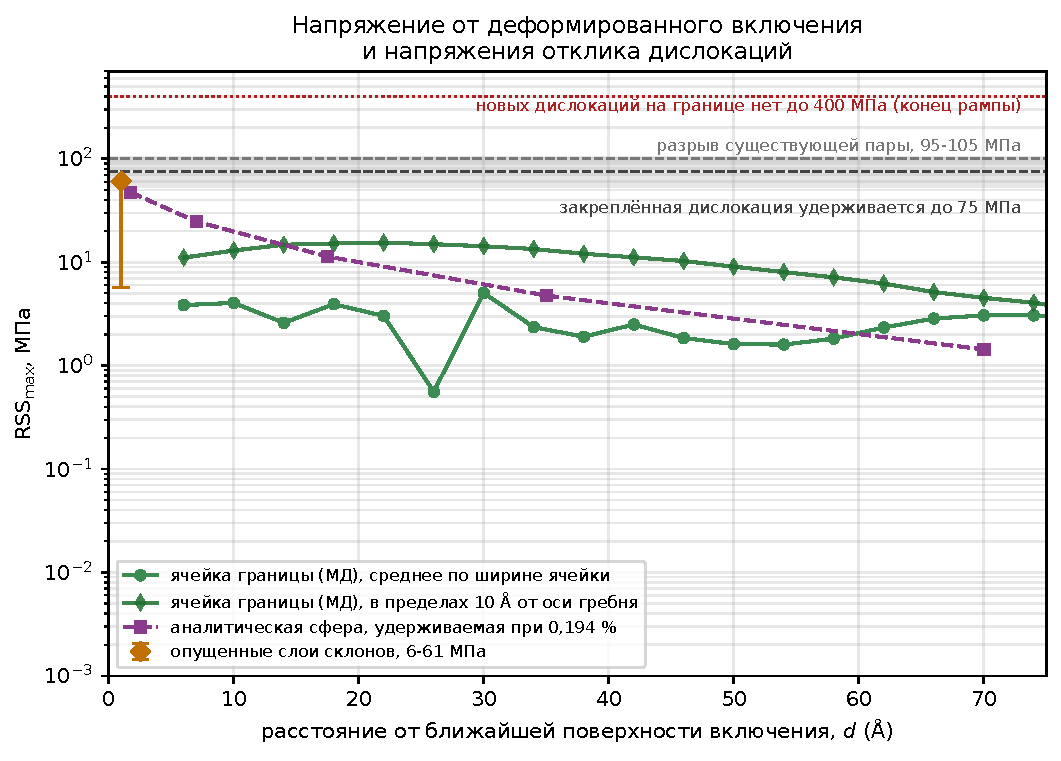
\includegraphics[width=0.9\linewidth]{fig_rss_vs_thresholds_ru}
\caption{Напряжение от деформированного включения и напряжения отклика
дислокаций: касательное напряжение, спроецированное на наиболее
благоприятную систему скольжения, $\mathrm{RSS}_{\max}$, в логарифмическом
масштабе в зависимости от расстояния $d$ до ближайшей поверхности
включения. Зелёные кружки --- ячейка границы (91\,428 атомов) с гребнем,
удерживаемым при 0{,}194\%, в среднем по ширине ячейки; зелёные ромбы --- то
же в пределах 10~\AA{} от оси гребня; для гребня $d = r - 20$~\AA{} (высота
вершины). Фиолетовые квадраты --- точное решение Эшелби [7] для сферического
включения радиуса $a = 35$~\AA{}, удерживаемого при том же удлинении в
бесконечной упругой матрице алюминия ($\mu = 26{,}5$~ГПа, $\nu = 0{,}347$,
объём-сохраняющее удлинение формулы~(1) с осью под 45$^\circ$ к $z$, тот же
максимум по двенадцати системам скольжения); для сферы $d = r - a$.
Горизонтальные линии --- конец рампы, 400~МПа, до которого новых
дислокаций на границе не образовалось (пунктир), и напряжение, при котором
приходит в движение существующая пара дислокаций (95--105~МПа), оба
из раздела~3.2; затенённая полоса $75 \pm 22$~МПа --- напряжение, выдерживаемое
закреплённой дислокацией раздела~3.3 (приложенные 75~МПа плюс-минус взаимное
напряжение пары 22~МПа с неустановленным знаком). Оранжевый ромб отмечает
диапазон, охватываемый опущенными слоями на склонах гребня; измерением поля
он не является.}
\label{fig:rss}
\end{figure}

\begin{figure}[!htbp]
\centering
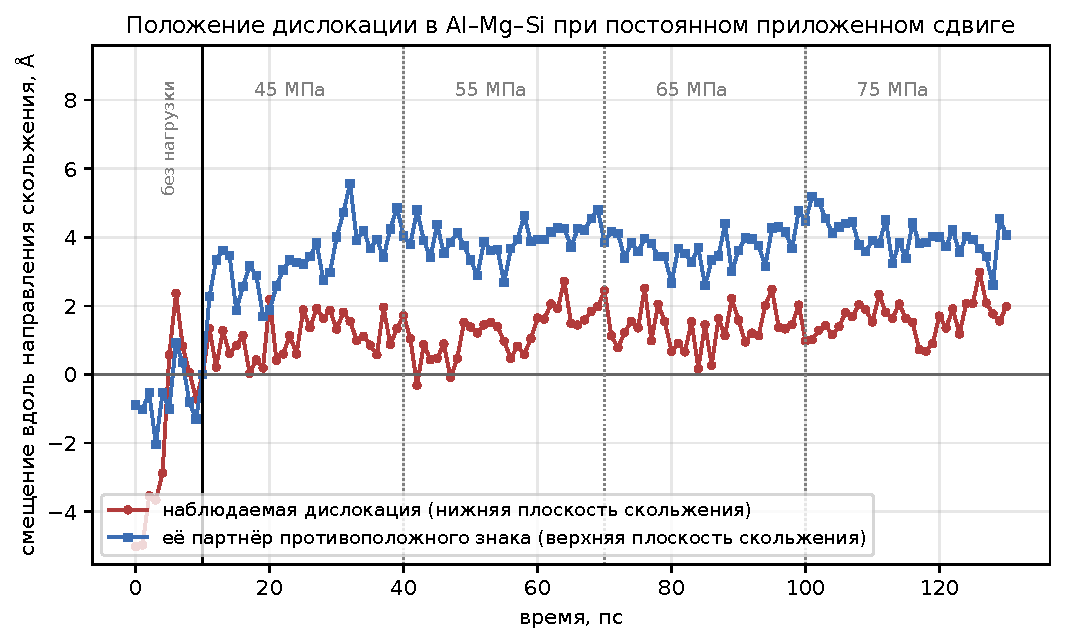
\includegraphics[width=0.9\linewidth]{fig_trajectories_ru}
\caption{Положение дислокации вдоль направления скольжения в зависимости от
времени в ячейке Al--Mg--Si при ступенчатом нагружении постоянными
приложенными сдвиговыми напряжениями (пунктир --- границы ступеней, над
каждой указано приложенное напряжение; смещение отсчитывается от положения в момент включения нагрузки,
$t = 10$~пс, после 10~пс без нагрузки). Красная кривая --- дислокация, за
движением которой велось наблюдение (нижняя в паре); синяя --- её партнёр
противоположного знака в верхней плоскости скольжения. Дислокация
колеблется около одного положения и не движется: пластического смещения
нет ни при одном из четырёх уровней напряжения. За всю историю нагружения
она смещается на 2{,}0~\AA{}, меньше одного вектора Бюргерса
$b = 2{,}86$~\AA{}, при амплитуде тепловых колебаний 0{,}6~\AA{}. Партнёр в
момент включения нагрузки выбирает 4{,}1~\AA{} ($1{,}4\,b$) и на этом
останавливается: за оставшиеся три ступени его положение меняется меньше,
чем на амплитуду его тепловых колебаний 0{,}5~\AA{}. Этот одиночный
начальный шаг не является устойчивым скольжением.
}
\label{fig:traj}
\end{figure}

\subsection{Подвижность дислокаций и закрепление примесями в сплаве}

Сопротивление, которое растворённые атомы Mg и Si оказывают движению
дислокации, измерено в ячейке сплава раздела~2.3: без включения, с
1{,}0~ат.\%~Mg и 0{,}6~ат.\%~Si, случайно замещающими алюминий, и с одной
парой краевых дислокаций противоположного знака в плоскостях скольжения,
отстоящих друг от друга на 206~\AA{}; ячейка нагружалась лестницей
постоянных приложенных сдвиговых напряжений 45, 55, 65 и 75~МПа по 30~пс
каждое. На рис.~\ref{fig:traj} показано положение дислокации, за движением
которой велось наблюдение (нижней в паре), и её партнёра в зависимости от
времени. Дислокация не скользит. За 120~пс нагружения она смещается на
2{,}0~\AA{} --- меньше одного вектора Бюргерса $b = 2{,}86$~\AA{} --- при
амплитуде тепловых колебаний 0{,}6~\AA{}; нетто-смещения внутри четырёх
ступеней, 0{,}6, 1{,}6, $-1{,}5$ и 0{,}2~\AA{} при 45, 55, 65 и 75~МПа,
сопоставимы с этими колебаниями и с напряжением не растут. Линия колеблется
около одного положения и при каждом уровне напряжения остаётся удержанной
окружающими её примесными атомами. Скорость, разумеется, можно подобрать
для каждой ступени, но при таких отношениях смещения к амплитуде колебаний
(все ниже 3) она описывала бы колебания, а не дрейф, и не приводится.
Траектория устанавливает нижнюю границу: выбранная случайная конфигурация
атомов Mg и Si удерживает дислокацию против движущего напряжения не менее
75~МПа. Это превышает 15~МПа, создаваемые удерживаемым гребнем у
своей поверхности (раздел~3.1), в 5 раз, а 41~МПа
аналитической сферы --- в 1{,}8 раза. Две дислокации пары действуют друг на
друга взаимным напряжением 22~МПа, знак которого относительно приложенного
сдвига здесь не установлен, поэтому осторожное прочтение границы ---
$75 \pm 22$~МПа с нижним краем 53~МПа, который всё ещё превышает обе
амплитуды. Граница лежит и выше оценки Лабуша
$\tau_c \approx 38$~МПа для данного содержания примесей [15,\,16] ---
среднеполевой оценки напряжения, необходимого, чтобы протащить дислокацию
сквозь случайное распределение примесных атомов, --- что согласуется с
локально более сильным, чем в среднем, расположением примесей в данной
единственной реализации.

В ячейке чистого алюминия той же геометрии дислокация движется свободно: её
положение блуждает в пределах отдельных ступеней напряжения на величину до
20~\AA{}, и за 130~пс траектории не происходит ни одного события захвата. В
рамках данной модели закрепление примесными атомами является, таким
образом, единственным представленным в этих ячейках препятствием движению
дислокаций. Количественный закон торможения дислокации в чистом алюминии
из той же геометрии получить не удалось: в отсутствие препятствий один из
членов пары достигает свободной поверхности и поглощается ею уже на первой
ступени, а блуждания оставшейся линии ограничены остаточным полем
периодической дислокационной конструкции; поэтому наблюдение закрепления в
сплаве сопоставляется с оценкой Лабуша, а не с измеренным коэффициентом
торможения. Поскольку открепления не происходит, активационный объём $V^{*}$ (объём, заметаемый сегментом дислокации при преодолении препятствия; он определяет, насколько сильно скорость скольжения откликается на напряжение) из этих расчётов извлечь нельзя. В качестве
центрального сценария используется $V^{*} = 70\,b^{3}$, полученное Soula и
соавт. для Al--Mg--Si после равноканального углового прессования [17];
поскольку состояние того материала отличается от рассматриваемого,
интервал $V^{*} = 19$--$142\,b^{3}$ [18] используется только как диапазон
чувствительности. Траектория служит лишь для оценки прочности препятствий
снизу. Кластеры Mg/Si не строились и не идентифицировались. Вторая случайная
конфигурация, рассчитанная только до ступеней 45, 55 и 65~МПа, точно так же
удерживала дислокацию на каждой достигнутой ступени; граница 75~МПа
опирается на ту единственную реализацию, которая прошла всю лестницу.